\documentclass{standalone}
\usepackage{tikz}
\usetikzlibrary{patterns, positioning}

\begin{document}
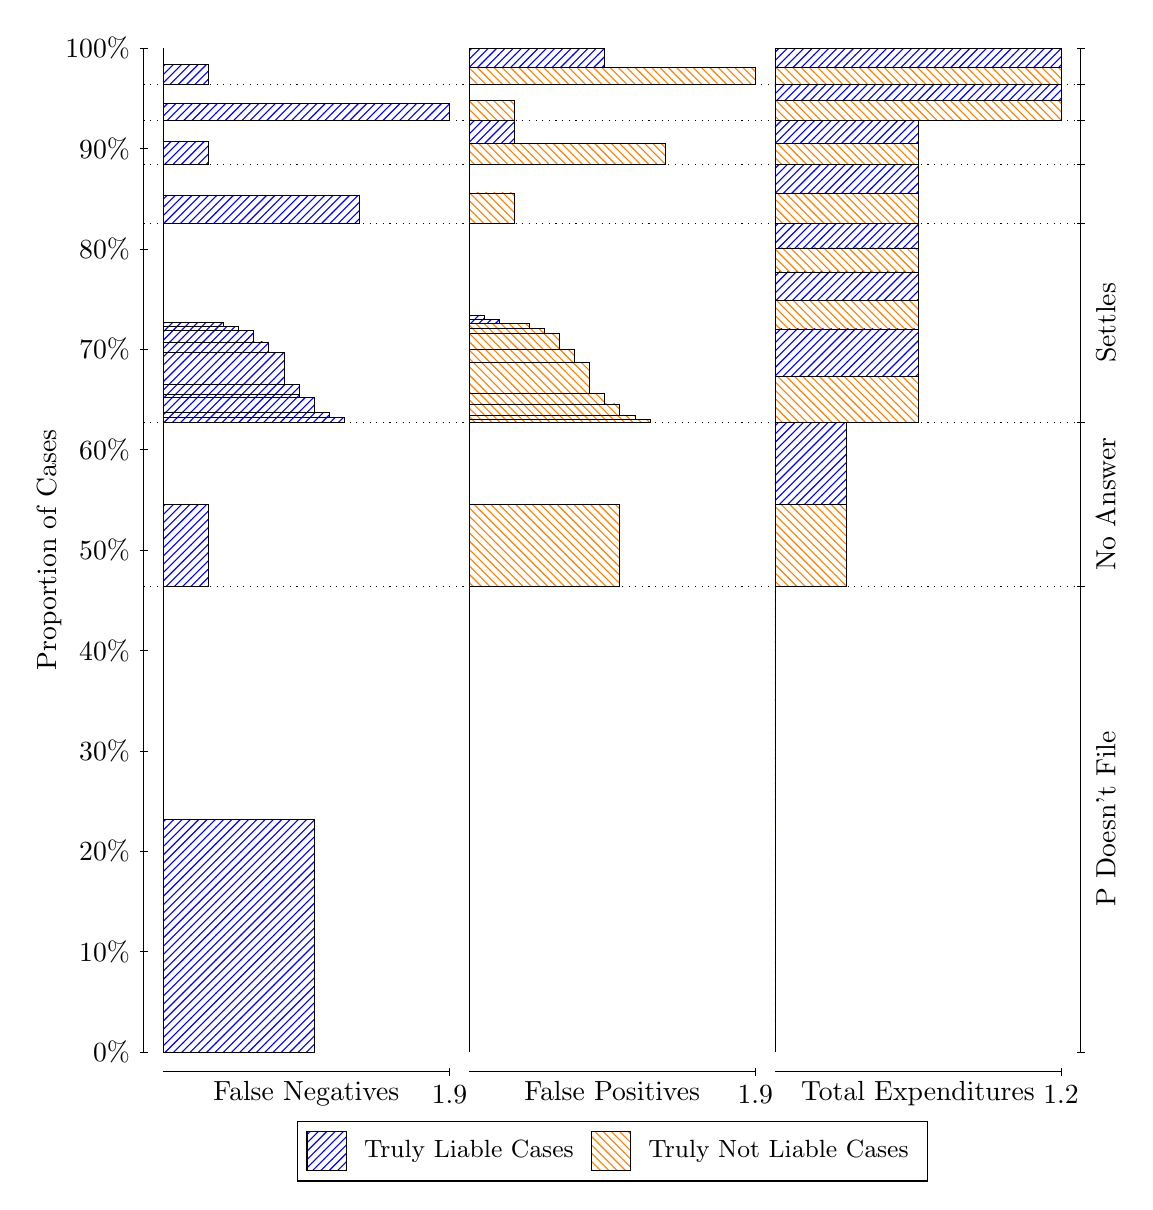
\begin{tikzpicture}
\draw[black, very thin] (1.5,1.75) -- (1.5,14.5);
\node[rotate=90, anchor=center] at (0.3, 8.125) {Proportion of Cases};
\draw[black, very thin] (1.45,1.75) -- (1.55,1.75);
\node[anchor=east] at (1.45, 1.75) {0\%};
\draw[black, very thin] (1.45,3.025) -- (1.55,3.025);
\node[anchor=east] at (1.45, 3.025) {10\%};
\draw[black, very thin] (1.45,4.3) -- (1.55,4.3);
\node[anchor=east] at (1.45, 4.3) {20\%};
\draw[black, very thin] (1.45,5.575) -- (1.55,5.575);
\node[anchor=east] at (1.45, 5.575) {30\%};
\draw[black, very thin] (1.45,6.85) -- (1.55,6.85);
\node[anchor=east] at (1.45, 6.85) {40\%};
\draw[black, very thin] (1.45,8.125) -- (1.55,8.125);
\node[anchor=east] at (1.45, 8.125) {50\%};
\draw[black, very thin] (1.45,9.4) -- (1.55,9.4);
\node[anchor=east] at (1.45, 9.4) {60\%};
\draw[black, very thin] (1.45,10.675) -- (1.55,10.675);
\node[anchor=east] at (1.45, 10.675) {70\%};
\draw[black, very thin] (1.45,11.95) -- (1.55,11.95);
\node[anchor=east] at (1.45, 11.95) {80\%};
\draw[black, very thin] (1.45,13.225) -- (1.55,13.225);
\node[anchor=east] at (1.45, 13.225) {90\%};
\draw[black, very thin] (1.45,14.5) -- (1.55,14.5);
\node[anchor=east] at (1.45, 14.5) {100\%};

\draw[black, very thin] (13.4,1.75) -- (13.4,14.5);
\draw[black, very thin] (13.35,1.75) -- (13.45,1.75);
\node[anchor=west] at (13.35, 1.75) {};
\draw[black, very thin] (13.35,7.6662) -- (13.45,7.6662);
\node[anchor=west] at (13.35, 7.6662) {};
\draw[black, very thin] (13.35,9.7446) -- (13.45,9.7446);
\node[anchor=west] at (13.35, 9.7446) {};
\draw[black, very thin] (13.35,12.274) -- (13.45,12.274);
\node[anchor=west] at (13.35, 12.274) {};
\draw[black, very thin] (13.35,13.02) -- (13.45,13.02);
\node[anchor=west] at (13.35, 13.02) {};
\draw[black, very thin] (13.35,13.582) -- (13.45,13.582);
\node[anchor=west] at (13.35, 13.582) {};
\draw[black, very thin] (13.35,14.041) -- (13.45,14.041);
\node[anchor=west] at (13.35, 14.041) {};
\draw[black, very thin] (13.35,14.5) -- (13.45,14.5);
\node[anchor=west] at (13.35, 14.5) {};

\draw[black, very thin, pattern color=blue, pattern=north east lines] (1.75,1.75) rectangle (3.6623,4.7081);
\draw[black, very thin, pattern color=orange, pattern=north west lines] (1.75,4.7081) rectangle (1.75,7.6662);
\draw[black, very thin, pattern color=blue, pattern=north east lines] (1.75,7.6662) rectangle (2.3237,8.7054);
\draw[black, very thin, pattern color=orange, pattern=north west lines] (1.75,8.7054) rectangle (1.75,9.7446);
\draw[black, very thin, pattern color=blue, pattern=north east lines] (1.75,9.7446) rectangle (4.0447,9.8059);
\draw[black, very thin, pattern color=blue, pattern=north east lines] (1.75,9.8059) rectangle (3.8535,9.8704);
\draw[black, very thin, pattern color=blue, pattern=north east lines] (1.75,9.8704) rectangle (3.6623,10.064);
\draw[black, very thin, pattern color=blue, pattern=north east lines] (1.75,10.064) rectangle (3.4711,10.103);
\draw[black, very thin, pattern color=blue, pattern=north east lines] (1.75,10.103) rectangle (3.4711,10.233);
\draw[black, very thin, pattern color=blue, pattern=north east lines] (1.75,10.233) rectangle (3.2798,10.633);
\draw[black, very thin, pattern color=blue, pattern=north east lines] (1.75,10.633) rectangle (3.0886,10.768);
\draw[black, very thin, pattern color=blue, pattern=north east lines] (1.75,10.768) rectangle (2.8974,10.916);
\draw[black, very thin, pattern color=blue, pattern=north east lines] (1.75,10.916) rectangle (2.7061,10.968);
\draw[black, very thin, pattern color=blue, pattern=north east lines] (1.75,10.968) rectangle (2.5149,11.013);
\draw[black, very thin, pattern color=orange, pattern=north west lines] (1.75,11.013) rectangle (1.75,12.274);
\draw[black, very thin, pattern color=blue, pattern=north east lines] (1.75,12.274) rectangle (4.236,12.633);
\draw[black, very thin, pattern color=orange, pattern=north west lines] (1.75,12.633) rectangle (1.75,13.02);
\draw[black, very thin, pattern color=blue, pattern=north east lines] (1.75,13.02) rectangle (2.3237,13.312);
\draw[black, very thin, pattern color=orange, pattern=north west lines] (1.75,13.312) rectangle (1.75,13.582);
\draw[black, very thin, pattern color=blue, pattern=north east lines] (1.75,13.582) rectangle (5.3833,13.792);
\draw[black, very thin, pattern color=orange, pattern=north west lines] (1.75,13.792) rectangle (1.75,14.041);
\draw[black, very thin, pattern color=blue, pattern=north east lines] (1.75,14.041) rectangle (2.3237,14.289);
\draw[black, very thin, pattern color=orange, pattern=north west lines] (1.75,14.289) rectangle (1.75,14.5);
\draw[black, very thin, pattern color=orange, pattern=north west lines] (5.6333,1.75) rectangle (5.6333,4.7081);
\draw[black, very thin, pattern color=blue, pattern=north east lines] (5.6333,4.7081) rectangle (5.6333,7.6662);
\draw[black, very thin, pattern color=orange, pattern=north west lines] (5.6333,7.6662) rectangle (7.5456,8.7054);
\draw[black, very thin, pattern color=blue, pattern=north east lines] (5.6333,8.7054) rectangle (5.6333,9.7446);
\draw[black, very thin, pattern color=orange, pattern=north west lines] (5.6333,9.7446) rectangle (7.9281,9.7874);
\draw[black, very thin, pattern color=orange, pattern=north west lines] (5.6333,9.7874) rectangle (7.7368,9.8372);
\draw[black, very thin, pattern color=orange, pattern=north west lines] (5.6333,9.8372) rectangle (7.5456,9.9807);
\draw[black, very thin, pattern color=orange, pattern=north west lines] (5.6333,9.9807) rectangle (7.3544,10.114);
\draw[black, very thin, pattern color=orange, pattern=north west lines] (5.6333,10.114) rectangle (7.1632,10.509);
\draw[black, very thin, pattern color=orange, pattern=north west lines] (5.6333,10.509) rectangle (6.9719,10.677);
\draw[black, very thin, pattern color=orange, pattern=north west lines] (5.6333,10.677) rectangle (6.7807,10.873);
\draw[black, very thin, pattern color=orange, pattern=north west lines] (5.6333,10.873) rectangle (6.5895,10.941);
\draw[black, very thin, pattern color=orange, pattern=north west lines] (5.6333,10.941) rectangle (6.3982,11.005);
\draw[black, very thin, pattern color=blue, pattern=north east lines] (5.6333,11.005) rectangle (6.0158,11.051);
\draw[black, very thin, pattern color=blue, pattern=north east lines] (5.6333,11.051) rectangle (5.8246,11.103);
\draw[black, very thin, pattern color=blue, pattern=north east lines] (5.6333,11.103) rectangle (5.6333,12.274);
\draw[black, very thin, pattern color=orange, pattern=north west lines] (5.6333,12.274) rectangle (6.207,12.661);
\draw[black, very thin, pattern color=blue, pattern=north east lines] (5.6333,12.661) rectangle (5.6333,13.02);
\draw[black, very thin, pattern color=orange, pattern=north west lines] (5.6333,13.02) rectangle (8.1193,13.289);
\draw[black, very thin, pattern color=blue, pattern=north east lines] (5.6333,13.289) rectangle (6.207,13.582);
\draw[black, very thin, pattern color=orange, pattern=north west lines] (5.6333,13.582) rectangle (6.207,13.831);
\draw[black, very thin, pattern color=blue, pattern=north east lines] (5.6333,13.831) rectangle (5.6333,14.041);
\draw[black, very thin, pattern color=orange, pattern=north west lines] (5.6333,14.041) rectangle (9.2667,14.252);
\draw[black, very thin, pattern color=blue, pattern=north east lines] (5.6333,14.252) rectangle (7.3544,14.5);
\draw[black, very thin, pattern color=orange, pattern=north west lines] (9.5167,1.75) rectangle (9.5167,4.7081);
\draw[black, very thin, pattern color=blue, pattern=north east lines] (9.5167,4.7081) rectangle (9.5167,7.6662);
\draw[black, very thin, pattern color=orange, pattern=north west lines] (9.5167,7.6662) rectangle (10.425,8.7054);
\draw[black, very thin, pattern color=blue, pattern=north east lines] (9.5167,8.7054) rectangle (10.425,9.7446);
\draw[black, very thin, pattern color=orange, pattern=north west lines] (9.5167,9.7446) rectangle (11.333,10.333);
\draw[black, very thin, pattern color=blue, pattern=north east lines] (9.5167,10.333) rectangle (11.333,10.933);
\draw[black, very thin, pattern color=orange, pattern=north west lines] (9.5167,10.933) rectangle (11.333,11.299);
\draw[black, very thin, pattern color=blue, pattern=north east lines] (9.5167,11.299) rectangle (11.333,11.658);
\draw[black, very thin, pattern color=orange, pattern=north west lines] (9.5167,11.658) rectangle (11.333,11.963);
\draw[black, very thin, pattern color=blue, pattern=north east lines] (9.5167,11.963) rectangle (11.333,12.274);
\draw[black, very thin, pattern color=orange, pattern=north west lines] (9.5167,12.274) rectangle (11.333,12.661);
\draw[black, very thin, pattern color=blue, pattern=north east lines] (9.5167,12.661) rectangle (11.333,13.02);
\draw[black, very thin, pattern color=orange, pattern=north west lines] (9.5167,13.02) rectangle (11.333,13.289);
\draw[black, very thin, pattern color=blue, pattern=north east lines] (9.5167,13.289) rectangle (11.333,13.582);
\draw[black, very thin, pattern color=orange, pattern=north west lines] (9.5167,13.582) rectangle (13.15,13.831);
\draw[black, very thin, pattern color=blue, pattern=north east lines] (9.5167,13.831) rectangle (13.15,14.041);
\draw[black, very thin, pattern color=orange, pattern=north west lines] (9.5167,14.041) rectangle (13.15,14.252);
\draw[black, very thin, pattern color=blue, pattern=north east lines] (9.5167,14.252) rectangle (13.15,14.5);
\draw[black, dotted] (1.5,7.6662) -- (13.4,7.6662);
\draw[black, dotted] (1.5,9.7446) -- (13.4,9.7446);
\draw[black, dotted] (1.5,12.274) -- (13.4,12.274);
\draw[black, dotted] (1.5,13.02) -- (13.4,13.02);
\draw[black, dotted] (1.5,13.582) -- (13.4,13.582);
\draw[black, dotted] (1.5,14.041) -- (13.4,14.041);
\draw[black, very thin] (1.75,1.5) -- (5.3833,1.5);
\node[anchor=north] at (3.5667, 1.5) {False Negatives};
\draw[black, very thin] (5.3833,1.45) -- (5.3833,1.55);
\node[anchor=north] at (5.3833, 1.45) {1.9};

\draw[black, very thin] (5.6333,1.5) -- (9.2667,1.5);
\node[anchor=north] at (7.45, 1.5) {False Positives};
\draw[black, very thin] (9.2667,1.45) -- (9.2667,1.55);
\node[anchor=north] at (9.2667, 1.45) {1.9};

\draw[black, very thin] (9.5167,1.5) -- (13.15,1.5);
\node[anchor=north] at (11.333, 1.5) {Total Expenditures};
\draw[black, very thin] (13.15,1.45) -- (13.15,1.55);
\node[anchor=north] at (13.15, 1.45) {1.2};

\node[black, centered, rotate=90] at (13.72, 4.7081) {P Doesn't File};
\node[black, centered, rotate=90] at (13.72, 8.7054) {No Answer};
\node[black, centered, rotate=90] at (13.72, 11.009) {Settles};





\draw (7.449999999999999,1.5) node[draw=none] (baseCoordinate) {};
\begin{scope}[align=center]
        \matrix[scale=0.5, draw=black, below=0.5cm of baseCoordinate, nodes={draw}, column sep=0.1cm]{
            \node[rectangle, draw, minimum width=0.5cm, minimum height=0.5cm, pattern=north east lines, pattern color=blue] {}; &
            \node[draw=none, font=\small] (B) {Truly Liable Cases}; &
            \node[rectangle, draw, minimum width=0.5cm, minimum height=0.5cm, pattern=north west lines, pattern color=orange] {}; &
            \node[draw=none, font=\small] (B) {Truly Not Liable Cases}; \\
            };
\end{scope}

\end{tikzpicture}
\end{document}